\chapter{Preliminary Studies}
\label{chap:prestudy}
\section{Children with asthma}
%%%%%%%%%%%%%%%%%%%%%%%%%%%%%%%%%%%%%%%%%%%%%%%%%%%%%%%%%%%%%%%%%%%%%%%%%%%%%%%%%Hva med en seksjon først generelt om astma, medisiner og medisineringsmetoder. Så mer direkte mot barn og astma. Og så la neste seksjon komme med problemene dette medfører (slik det er nå).
%%%%%%%%%%%%%%%%%%%%%%%%%%%%%%%%%%%%%%%%%%%%%%%%%%%%%%%%%%%%%%%%%%%%%%%%%%%%%%%%%
Asthma is a chronic inflamatory disease that affects the airways and lungs.\cite{naafastma} It is often more prominent in children, who are more 
active and easily excited than adults. The asthma is typically triggered by excitement, physical activity, rashes or allergies. The problem is 
managed by multiple medicines, 
with different schedules as to when to take them, and how much to take, depending on the condition of the child. There are inhalation medicines that 
consists of either small dust particles that effect the lungs locally, or saltwater that are inhaled as vapor, either alone or combined with other 
medicines to loosen up slime. Among these inhalation medicines is Ventoline and Flutide, seen in figure \ref{fig:ventoline} and \ref{fig:flutide}. 
There are also pills and liquid medicines that either affects the immune system or affects the body globally, not just locally in the lungs.

\begin{figure}
	\begin{minipage}[b]{0.4\linewidth}
		\centering
			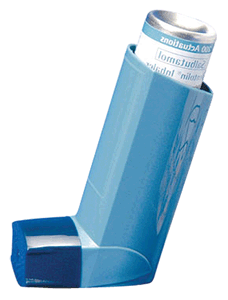
\includegraphics[width=0.15\paperwidth]{Pictures/ventoline}
		\caption[Ventoline]{Ventoline\cite{ventoline} is an inhalation medicine that opens up the airways shortly after inhaling it.}
		\label{fig:ventoline}
	\end{minipage}
	\hspace{3cm}
	\begin{minipage}[b]{0.4\linewidth}
		\centering
			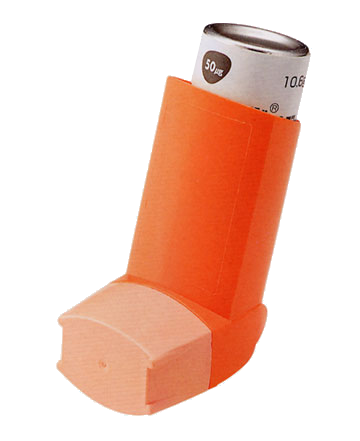
\includegraphics[width=0.15\paperwidth]{Pictures/flutide}
		\caption[Flutide]{Flutide is a steroid keeping the illness checked, but it has no immediate effect.}
		\label{fig:flutide}
	\end{minipage}
\end{figure}

The medicines can also be divided into medicines that have immediate effects, and are used during an asthma attack, while other medicines are preventative, 
and is taken on a regular schedule. These preventative medicines are targeted at bolstering your immune system before going to certain areas, or days
where the child is likely to be in contact with materials it is allergic to.	

With some of the inhalation medicines it's difficult to time the inhalation with the release of medicine, and here an inhalation chamber, or inhalation 
mask, is used. When the child has taken the nebulizer this way, usually once or twice a day, they must remember to wash their mouth afterwards.

Figure \ref{fig:paperprototype} shows an image of a nebulizer machine. The nebulizer machines often makes alot of noise, and can 
be scary to children. The nebulizer treatment takes between 2-10 minutes, 1-4 times a day.

\begin{figure}[t]
	\center
		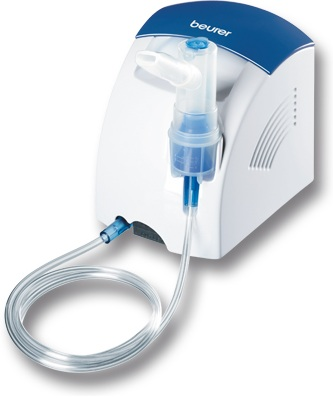
\includegraphics[width=0.4\linewidth]{Pictures/nebulizer}
	\caption[A Nebulizer machine]{A nebulizer machine.\cite{nebulizer}}
	\label{fig:paperprototype}
\end{figure}

\subsection{Traffic Light Classification of Asthma Condition}
\label{sec:trafficlight}

The traffic light program is a way of classifying condition and resulting medication for asthmatic 
patients. It is a very simple system that requires very little knowledge to understand, and is 
therefore well-suited for a project aimed at children. The basic outline can be compared to a traffic
light.

Borge et al. (2002)\cite{livingwithasthma} defines the zones as \emph{green}, \emph{orange}, and \emph{red}
and describes effects and treatment for each of them.

\subsubsection{Green Zone}
Green is the normal zone. A patient in the green zone can be described as in ``regular condition''. 
He or she is breathing normally, even when doing light physical exercise.

When an asthmatic is the green zone, it is normal to take two to three different medicines each day,
often with cortisone

\subsubsection{Yellow Zone}
Yellow is the ``ill'' zone. When a patient is in the yellow zone, they exhibit moderate signs of illness
such as breathlessness and coughing. There may also be allergy reactions, and waking up at night from
breathlessness and coughing. A patient may be defined as being in the yellow zone if he or she has a cold.

In the yellow zone, patients typically take more medication than in the green zone. A normal amount
is 4 to 6 doses daily. The medication from the green plan is taken as normal, in addition to any new
medicines introduced by the yellow state.

\subsubsection{Red Zone}
The red zone is labeled the ``stop'' zone. A patient in the red zone will have almost closed airways,
making it very difficult to breathe and the person will have to stop any activities.

A patient in the red zone has to fix his or her state immediately. This could be by opening windows,
finding a good resting position, taking specific emergency medication or using specific breathing
techniques. If these courses of action don't help, the patient should immediately call the doctor. 

\section{Parents with children affected by asthma}

Parents of children with asthma face a series of challenges concerning the medication of their children. 
One of these challenges is to give the correct amount of medicine, the right type of medicine, at the 
correct time of the day. Many parents have experienced stressful mornings where they are late for work, 
their children are unwilling to take their medicine and they either do it in an incorrect manner, reducing the 
medicines effect, or not giving it at all. The medication plans can be hard to understand, even though they are 
designed to be easy, and it's typically only one of the parents that have been given the instructions from 
the doctor directly, making it even harder for the other one to do it correctly.

The children are not always happy about taking their medicine. The inhalation mask might be scary, the 
medication might interfere with their planned activities that day, or any number of other reasons the child 
might not want to take his/her medicine that day. Having to force a child to take their medicine could make the 
child associate taking the medicine with a negative experience, and it becomes increasingly difficult to 
give the medicine to the child. 

\section{The concept of gamification}

Gamification is the concept of applying game-design thinking to non-game applications to make them more fun 
and engaging. Nick Pelling (2011)\cite{pellingblog} writes that the term \emph{gamification} was introduced
in 2002, but was not popular before 2010 (Daniels, 2010\cite{danielsblog}).

Common techniques applied to introduce gamification to a process include, but are not limited to:
\begin{itemize}
  \item Achievements/badges
  \item Levels
  \item Leaderboards
  \item Progress bars
  \item Avatars
  \item Gifting
  \item Challenges
  \item Embedding of minigames
\end{itemize}

These techniques are all widely used. Here are some examples:
% footnote / bibliography alle
\begin{itemize}
  \item In games for platforms like Playstation and Xbox, gamification is frequently used
   to make people finish campaigns.(Hamari et.al, 2011\cite{trophies}) Trophies and achievements are used to motivate people to complete games 100\%. 
   You may have to collect every single item in the game, fight every boss and so on.
  \item Nike+ introduced gamification to training. (Zichermann et. al, 2011\cite{gamificationByDesign}) You can track how fast you run, your maximum pulse and so on, 
  and try to beat this target the next time you are running.
  \item You can ``check in'' to places you have been with Google Maps, Facebook, Foursquare, Google+, GoWalla, and similar applications.  
  \item Airline companies uses bonus points as motivation for customers to fly more with a company. (Gamification Wiki, 2012\cite{freqflyer}) At a certain 
  level of these points, you may get one more flight for free, get a free upgrade to a better seat and so on. 
\end{itemize} 

%Kanskje skrive om dette?
We hope gamification will help making children's treatment as enjoyable as possible. Michael 
Wu has proven that gamification has an impact on human motivation. Wu presents: ``Game 
mechanics and game dynamics are able to positively influence human behavior 
because they are designed to drive the players above the activation threshold (i.e. the upper 
right of the ability-motivation axis), and then trigger them into specific actions'' (Wu, 2011)\cite{gamification101}.  

The gamification elements most suited for children, is gifting and embedding of minigames. The gifting needs to be visual, and
the two elements can be interwoven to increase the effect, where the minigames changes according to what gifts you've already
achieved. Another way that can implement gifting targeted at children, is to implement a currency system, for example coins, and reward them
with physical rewards when they reach a certain amount of coins. The rewards could be all from small toys and candy, to larger items, depending
on the amount of coins, and the tasks performed to get the coins. A point here is to make sure the currency is very visual, to make sure even
young children understand how many coins they have.
The implementation of minigames would help greatly in distracting children during tedious tasks like nebulization treatments.

Gamification has a lot of positive sides, but it may have bad sides if gamification is done the wrong way.
The fact that we are using gamification to motivate children, makes this an even more serious concern. If children feel that
they are stuck in a game, motivation may very easily be broken down. So whatever concept we come up with, it has to be 
to motivate the children at all time. They cannot feel stuck with our app. This concept is up to the customer to create, 
while we will be implementing it.  

As written above, gamification may have negative effects on users. Anderson-Rainie (2012)\cite{andersonrainie} show results
that users are likely to not be motivated or feel that they are manipulated into completing a task. The 
research also show that users are likely to feel that gamification is too childish, and that gamification 
is a trend that will disappear within a few years. 

\section{Karotz}
Karotz.com (2012)\cite{karotz} describes Karotz as a robot shaped 
as a bunny that can interact with
a user through light, ear movement and sound. It can also take
input through a button, moving its ears, an RFID (Radio-frequency identification) chip, voice
commands and serial (Internet) communication.

The project includes developing an application for the Karotz
platform that will serve as an addition to the mobile applications.
It is therefore necessary to study its interfaces, development
methods and API of the machine.

\begin{figure}[h]
	\centering
		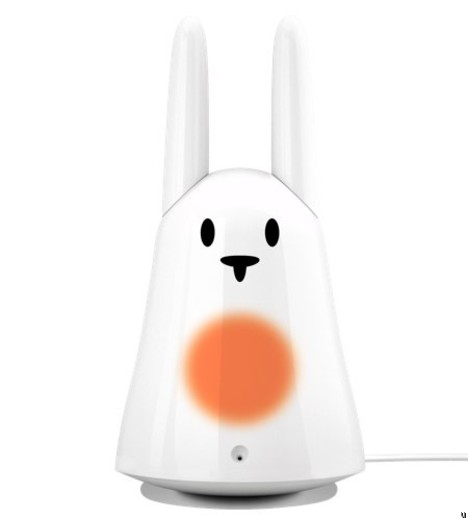
\includegraphics[height=10cm]{Pictures/karotzimg}
	\caption{Karotz: A bunny-shaped robot}
	\label{fig:karotz}
\end{figure}

\subsection{Application Platform}
Karotz application (called ``Appz'') are installed through an
online platform located on the Karotz web site. They can be
launched on the Karotz itself either through a scheduler, voice
commands or an RFID chip. These RFID chips come in various shapes,
sizes and colors. Figure \ref{fig:flatnanoz} and Figure 
\ref{fig:nanoztag} show examples of the different kinds of ``nanoz'',
that are small figures with an integrated RFID chip.

\begin{figure}
	\begin{minipage}[b]{0.4\linewidth}
		\centering
			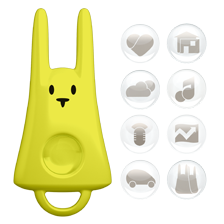
\includegraphics[width=0.30\paperwidth]{Pictures/FlatnanozYellow}
		\caption[Flatnanoz]{A flat nanoz--flatnanoz-- a figure with an RFID chip used to provide input to a Karotz.}
		\label{fig:flatnanoz}
	\end{minipage}
	\hspace{3cm}
	\begin{minipage}[b]{0.4\linewidth}
		\centering
			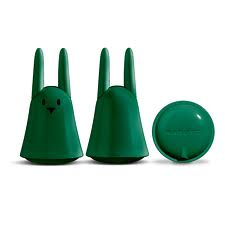
\includegraphics[width=0.30\paperwidth]{Pictures/NanoztagGreen}
		\caption[Nanoztag]{A round nanoz--nanoztag-- a figure with an RFID chip used to provide input to a Karotz.}
		\label{fig:nanoztag}
	\end{minipage}
\end{figure}

Some mentionable applications made by other developers are 
``At Home'', an application that may register that someone checks 
in at the Karotz, and send an e-mail to a predetermined mail 
address, so children may tell their parents that they are home. 
``Twitter for Karotz'' may read you tweets and post tweets based 
on voice-commands. Another mention is ``Weather'' which may tell 
you the forecast for the day or the following day. It seems all 
applications registered at the Karotz website are fairly simple 
and have little functionality.

As for launching the BLOPP application, the times for the scheduler must
be manually set through the Karotz web site, so it cannot be 
used for notifications directly. The best option for the BLOPP 
implementation would therefore be to set a scheduler to start
every day at 00:00 and stop every day at 23:59. This way it can
be ensured that the application is always running, updating
itself with medications, status and times, and a timer can be
used to schedule notifications.

%\subsection{The two APIs}
The Karotz can be programmed in two different ways: either
through a web REST (Representational State Transfe) framework, 
or with JavaScript that runs as an embedded program on the robot itself.

The requirement that a REST program would have to be hosted
somewhere, combined with the fact that an embedded program 
provides more flexibility in terms of local storage to limit the
amount of information sent over a network makes the JavaScript
framework a more suitable choice for the BLOPP project.

%\subsection{Karotz Output Channels}
The Karotz has a few ways of providing output to the end-user. It
can be asked to
\begin{itemize}
    \item play sound files;
    \item move its ears;
    \item speak, using a TTS (text-to-speach) engine;
    \item illuminate its stomach in different colors;
    and
    \item communicate over the internet with HTTP (Hyper Text Transfer Protocol) GET and POST 
          methods.
\end{itemize}

For providing user commands, TTS could be an option if the engine
supported Norwegian, but since the language options are limited to
English, French, German and Spanish, speech will have to be
created by recording sound files and playing them with the
multimedia engine.

\section{Pollen forecast}
\label{sec:pollencast}
NAAF\cite{naafasthma} states that asthma- and pollen treatment needs to be seen in correlation.
Children may feel worse during pollen season than the rest of the year. We intend to give parents more analyzing tools by being able to see
connections between asthma symptoms and different types of pollen by using pollen data. It may occur that asthma is not the original source of 
a child's condition, but an allergy against a certain pollen is the source.  
NAAF hosts a pollen forecast at \url{http://pollenvarslingen.no/} which we intend to use. We have been given a user key for this cast, even though
they do not normally distribute this sort of information to application developers.
\section{Design workshop}
\label{sec:designWorkshop}
Before the first sprint, a design workshop was held. Hanne Linander, a
master student in Industrial Design at NTNU was responsible for the workshop.
The goal was to come up with different ideas for functionality and design, and
make an early sketch for the layout of the application.

At this stage in the study, we had not yet decided to develop two separate
applications, so we created layout suggestions for an application aimed to do
both tasks for children and for adults.

Many different exercises were completed throughout the day, in order to make as many
creative ideas as possible. Examples of exercises are short time boxed sketch
sessions, cross-collaboration without explaining thoughts behind the sketches,
different idea-competitions, among others. At the end the ideas were evaluated,
resulting in many discards and some being taken into further development.
After the workshop the sketches and the ideas were presented to the customer.
The development team was very happy about the results and decided to develop a
paperprototype from the sketches.

\subsection{Results}
We drew several sketches of how we envisioned the different views in an 
imagined Android application. 

Figure \ref{fig:dwMainMenu} shows a suggestion for the main menu in the 
application, where the action of taking medicine is in focus. The menu includes:
\begin{itemize}
  \item a log button where an adult can view medication history for the child,
  \item a manual button for learning how to use medication,
  \item a settings button for adjusting mediation schedule, alarm ringtone etc.,
  \item an ``about the app'' button for learning how to use the application,
  \item a display where one can view the current health state for the child, and
  		also click on it to change the health state, and
  \item a count of how many stars the child has collected, with the option to
  		click on that count to see more detailed information about the rewards
  		collected.
\end{itemize}

Figure \ref{fig:dwHealthState} illustrates how a user would see the health state
view separately from the menu. It would consist of three elements represented as
colored smileys; one for each health state. The healthy smiley would be green and
smiling, the sick one would be yellow and in a mellow mood, while the very sick
state would be represented by a red, frowning smiley. The currently active health
state could be displayed by illuminating the respective smiley, and clicking on
another would change the active state.

Figure \ref{fig:dwHealthStatePopup} shows how the health state view could be 
integrated into the main menu better by injecting it into an overlay. This could
make navigating the app more intuitive.

Figure \ref{fig:dwMediationView} is an image of the view a user would first see
when clicking the big ``medicine'' button in the main menu, or the view he or she
sees when redirected from a notification. It shows an image of the medicine to be
taken, and gives the option to go directly to the medication process through
clicking on the medicine image itself. If a user is unsure about how to use the
medication, there is illustrated an option where one would directly be brought to
the manual page for that medicine.

Figure \ref{fig:dwPickChild} shows a view one would be brought to if more than one
child was registered in one application. It shows an icon for each child and the
child's name. Clicking one one or the other would bring the user to the distraction
page for that child.

Figure \ref{fig:dwMediationViewCloudsThunderstorm} is an image of the first part of
the distraction animation a child would see. It shows dark clouds and a thunderstorm
that represents the child's state before taking medication. It was thought of as a 
way to motivate children to take medication in order to clear up the clouds, and as
something children could relate to by comparing their progress to the clouds.

Figure \ref{fig:dwMediationViewEmergingMedicine} is also part of the distraction
animation. It shows a medicine unit emerging from behind the clouds which are clearing
up while the medication is ongoing. The emerging medication was supposed to symbolize
the goodness of medication, while the clearing of clouds would symbolize the child's
lungs and airways clearing up.

Figure \ref{fig:dwChildRewardsView} illustrates how a child could view his or her
collected stars. There is a big star with a count next to it, which would show the 
total amount of stars. In addition, there is a scrolling view on the top where each
day would have an amount of stars on it, corresponding to how many stars the child had
received on that day. Lastly, there is an appealing figure on the page, in this case
a ``ninja master'', which would be an avatar for the child. It was imagined as
something that the child would purchase or obtain after reaching a certain amount of stars,
and the object itself would vary, serving as an additional motivational factor to
supplement the stars themselves.

Figure \ref{fig:dwAdultLogView} is a view where adults could check the progress and
medication history for a child. It would display graphs of condition and how good they
were at following a medication plan. Days would be colored after what condition the 
child was in on that day. The amount of stars the child collected is also shown in each
day, and a percentage of how often a given medicine is taken on the planned time is
displayed on the bottom right.

\begin{figure}
	\begin{minipage}[b]{0.46\linewidth}
		\centering
			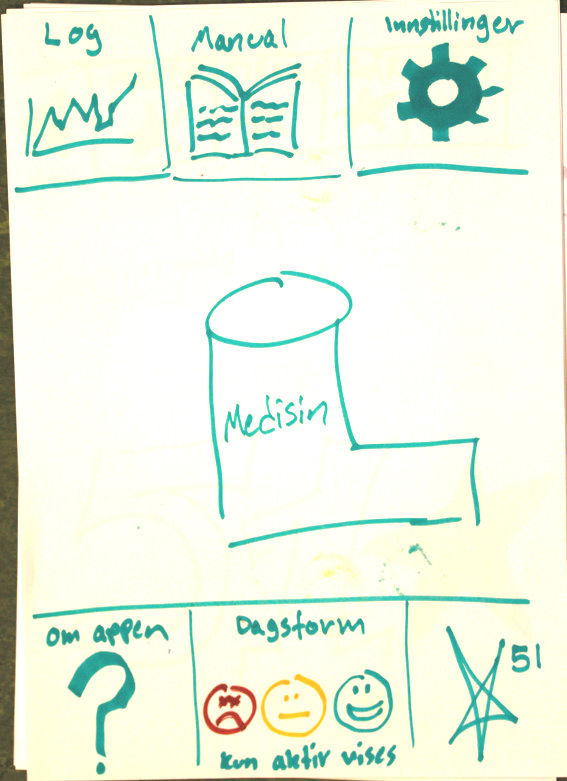
\includegraphics[width=0.34\paperwidth]{Pictures/DesignWorkshop/MobileMainMenu}
		\caption[Main menu view from design workshop]{View for the main menu of the application.}
		\label{fig:dwMainMenu}
	\end{minipage}
	\hspace{1cm}
	\begin{minipage}[b]{0.46\linewidth}
		\centering
		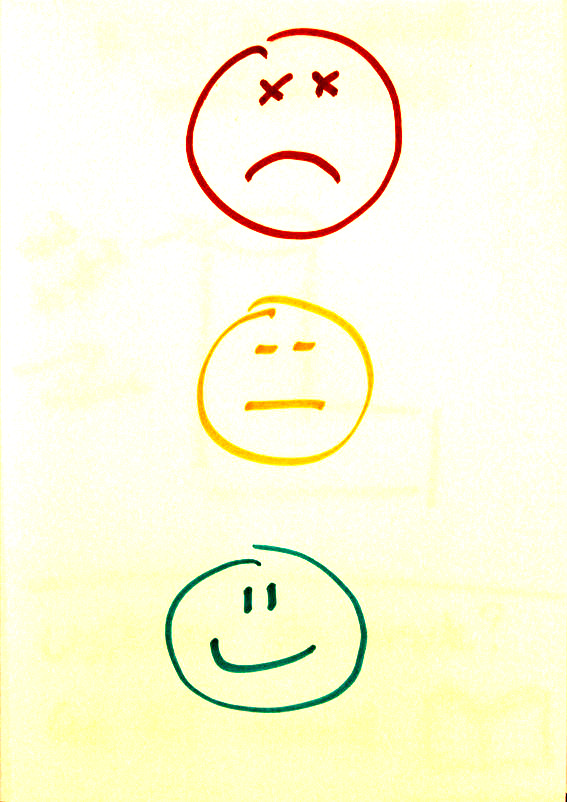
\includegraphics[width=0.34\paperwidth]{Pictures/DesignWorkshop/HealthStateView}
	\caption[Change health state view from design workshop]{View for changing health state (active medication plan).}
	\label{fig:dwHealthState}
	\end{minipage}
\end{figure}

% \begin{figure}
% 	\begin{center}
% 		\includegraphics[width=7cm]{}
% 		\caption{View for the main menu of the application.}
% 		\label{fig:dwMainMenu}
% 	\end{center}
% \end{figure}

% \begin{figure}
% 	\begin{center}
% 		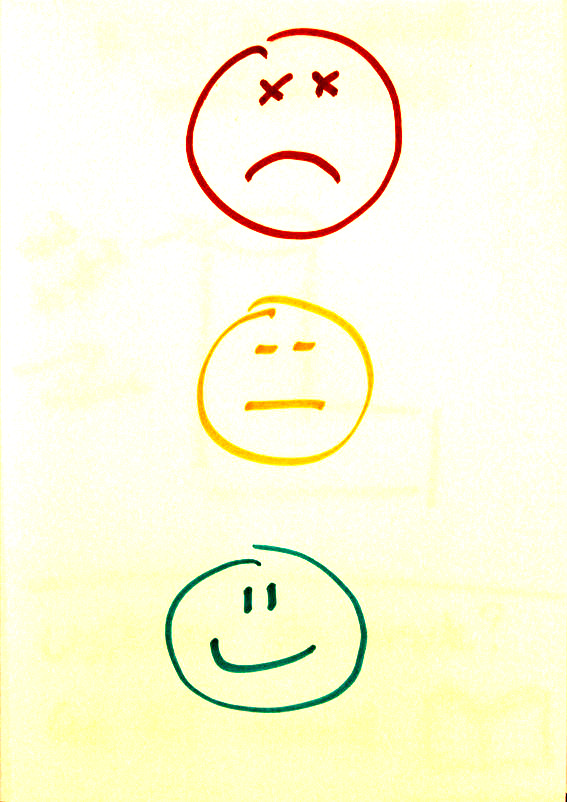
\includegraphics[width=7cm]{Pictures/DesignWorkshop/HealthStateView}
% 		\caption{View for changing health state (active medication plan).}
% 		\label{fig:dwHealthState}
% 	\end{center}
% \end{figure}

\begin{figure}
	\begin{minipage}[b]{0.46\linewidth}
		\centering
			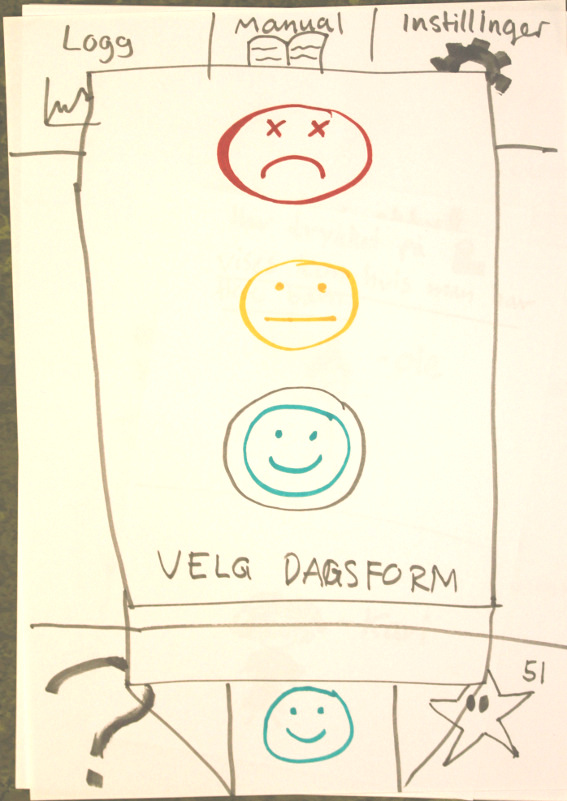
\includegraphics[width=0.34\paperwidth]{Pictures/DesignWorkshop/HealthStateViewPopup}
		\caption[Change health state as pop up from design workshop]{View for changing health state as a pop up from the main menu.}
		\label{fig:dwHealthStatePopup}
	\end{minipage}
	\hspace{1cm}
	\begin{minipage}[b]{0.46\linewidth}
		\centering
		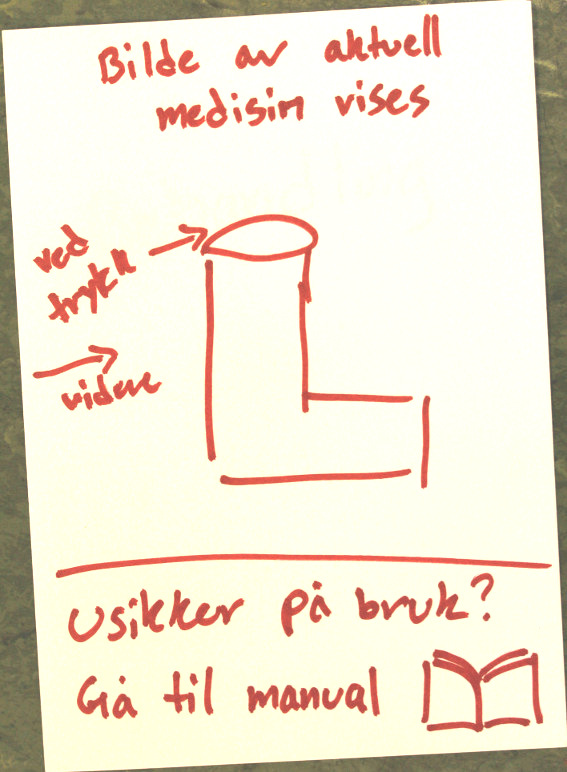
\includegraphics[width=0.34\paperwidth]{Pictures/DesignWorkshop/MedicationView}
	\caption[Start medication view from design workshop]{View for starting a medication and distraction process.}
	\label{fig:dwMediationView}
	\end{minipage}
\end{figure}

% \begin{figure}
% 	\begin{center}
% 		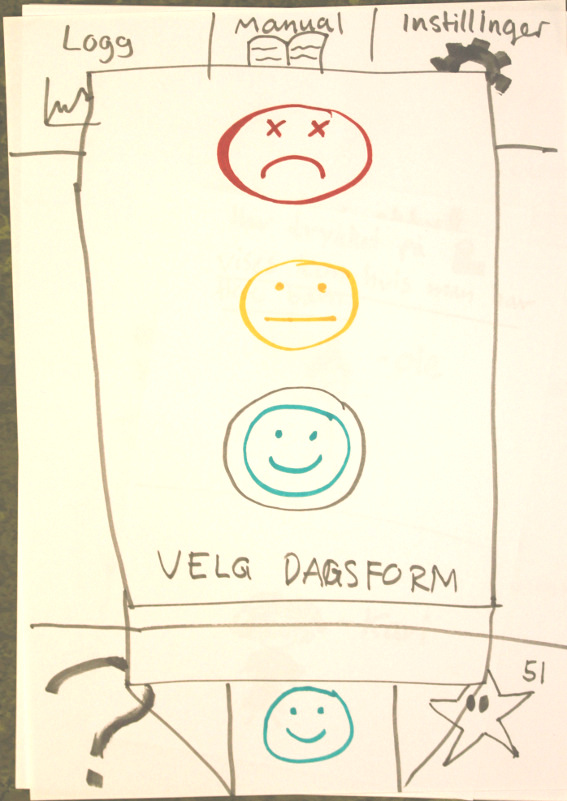
\includegraphics[width=7cm]{Pictures/DesignWorkshop/HealthStateViewPopup}
% 		\caption{View for changing health state as a popup from the main menu.}
% 		\label{fig:dwHealthStatePopup}
% 	\end{center}
% \end{figure}
% 
% \begin{figure}
% 	\begin{center}
% 		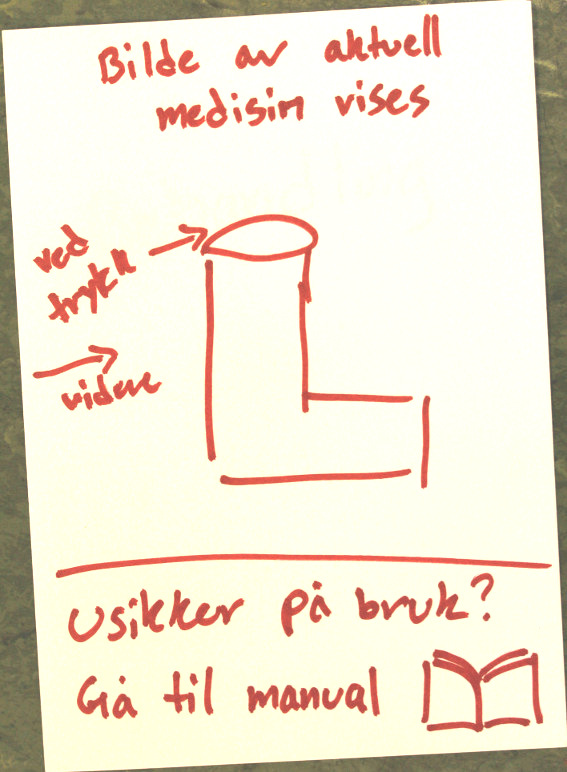
\includegraphics[width=7cm]{Pictures/DesignWorkshop/MedicationView}
% 		\caption{View for starting a medication and distraction process.}
% 		\label{fig:dwMediationView}
% 	\end{center}
% \end{figure}

\begin{figure}
	\begin{minipage}[b]{0.46\linewidth}
		\centering
			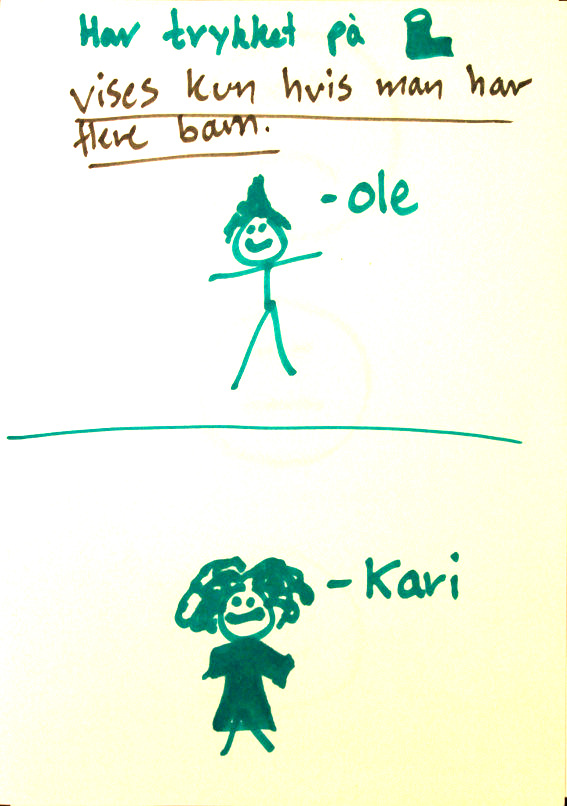
\includegraphics[width=0.34\paperwidth]{Pictures/DesignWorkshop/MedicationViewPickChild}
		\caption[Pick child view from design workshop]{View for choosing child to medicate at the start of medication mode.}
		\label{fig:dwPickChild}
	\end{minipage}
	\hspace{1cm}
	\begin{minipage}[b]{0.46\linewidth}
		\centering
		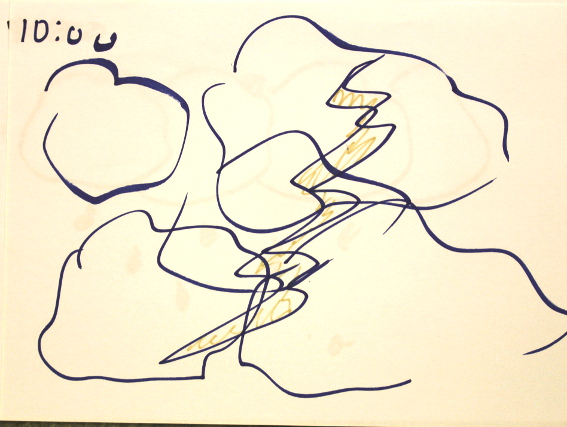
\includegraphics[width=0.34\paperwidth]{Pictures/DesignWorkshop/MedicationViewCloudsThunderstorm}
	\caption[Distraction view from design workshop]{Initial view of a distraction. Heavy clouds and thunderstorms represent the child's state before taking medicine.}
	\label{fig:dwMediationViewCloudsThunderstorm}
	\end{minipage}
\end{figure}

% \begin{figure}
% 	\begin{center}
% 		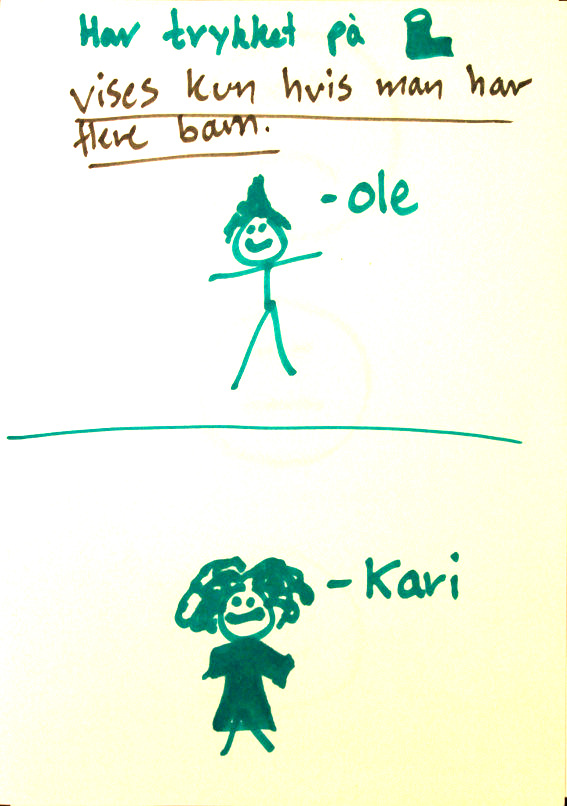
\includegraphics[width=7cm]{Pictures/DesignWorkshop/MedicationViewPickChild}
% 		\caption{View for choosing child to medicate at the start of medication mode.}
% 		\label{fig:dwPickChild}
% 	\end{center}
% \end{figure}
% 
% \begin{figure}
% 	\begin{center}
% 		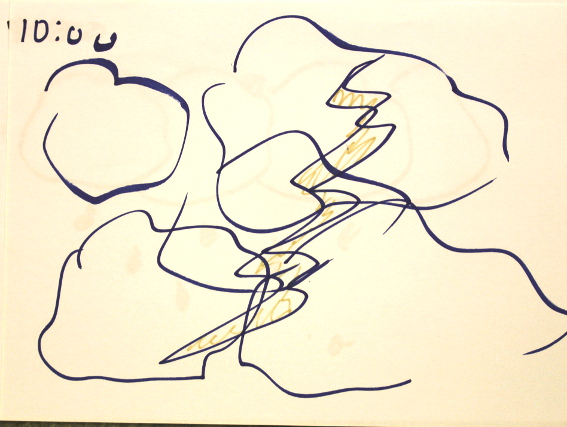
\includegraphics[width=7cm]{Pictures/DesignWorkshop/MedicationViewCloudsThunderstorm}
% 		\caption{Initial view of a distraction. Heavy clouds and thunderstorms represent the child's state before taking medicine.}
% 		\label{fig:dwMediationViewCloudsThunderstorm}
% 	\end{center}
% \end{figure}

\begin{figure}
	\begin{minipage}[b]{0.46\linewidth}
		\centering
			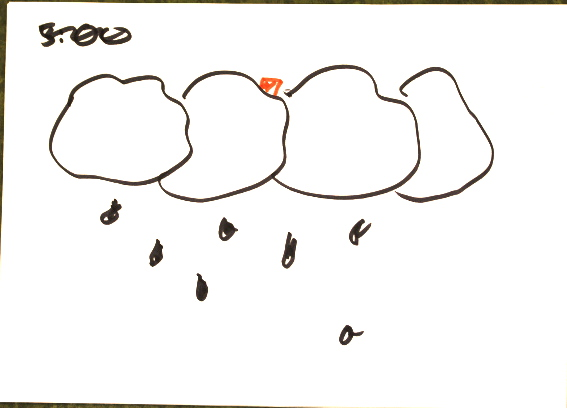
\includegraphics[width=0.34\paperwidth]{Pictures/DesignWorkshop/MedicationViewEmergingMedicine}
		\caption[Distraction view 2 from design workshop]{Subsequent view of a distraction process. The medication is emerging while the clouds are disappearing, to symbolize the healing effects of medicine.}
		\label{fig:dwMediationViewEmergingMedicine}
	\end{minipage}
	\hspace{1cm}
	\begin{minipage}[b]{0.46\linewidth}
		\centering
		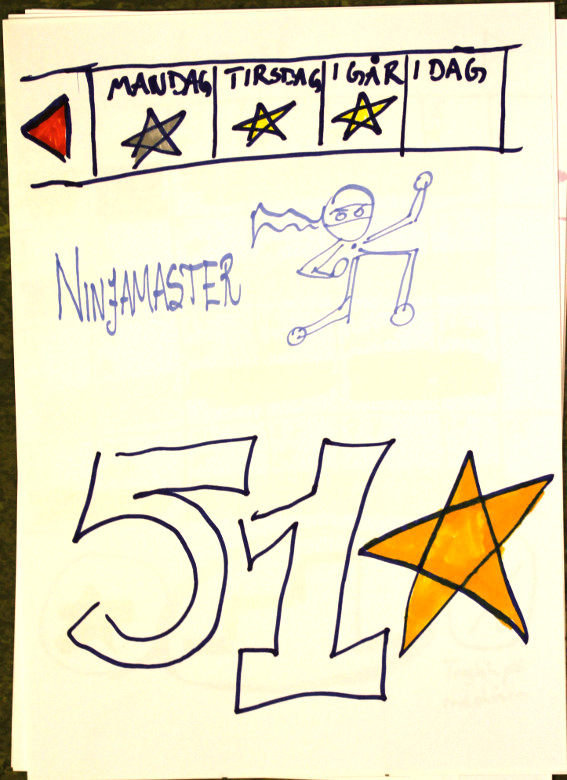
\includegraphics[width=0.34\paperwidth]{Pictures/DesignWorkshop/ChildRewardsView}
	\caption[Rewards view from design workshop]{View where children can view their collected reward (stars), and an acquired rank (in this case ``ninja master'').}
	\label{fig:dwChildRewardsView}
	\end{minipage}
\end{figure}

% \begin{figure}
% 	\begin{center}
% 		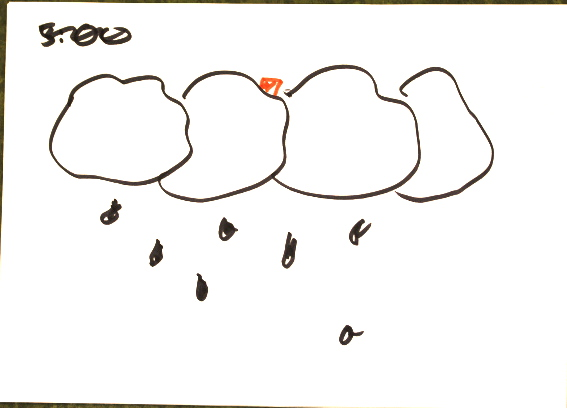
\includegraphics[width=7cm]{Pictures/DesignWorkshop/MedicationViewEmergingMedicine}
% 		\caption{Subsequent view of a distraction process. The medication is emergin while the clouds are disapeparing, to symbolize the healing effects of medicine.}
% 		\label{fig:dwMediationViewEmergingMedicine}
% 	\end{center}
% \end{figure}
% 
% \begin{figure}
% 	\begin{center}
% 		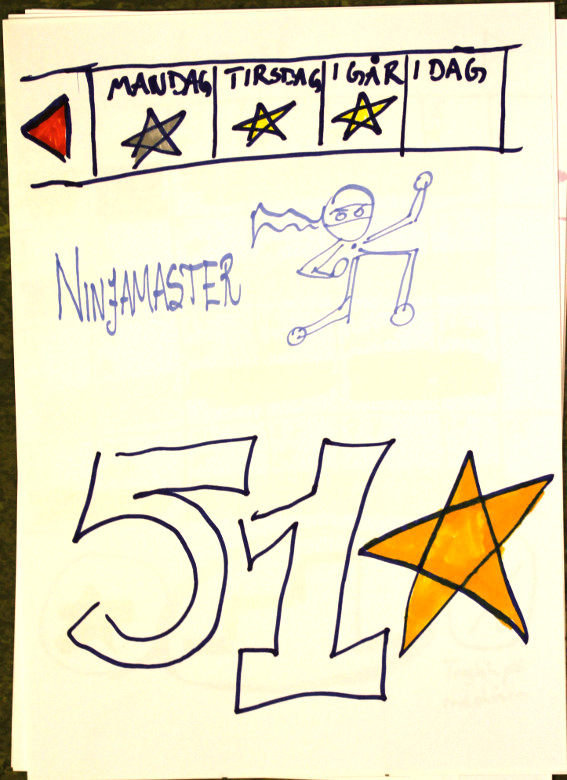
\includegraphics[width=7cm]{Pictures/DesignWorkshop/ChildRewardsView}
% 		\caption{View where children can view their collected reward (stars), and an acquired rank (in this case ``ninja master'').}
% 		\label{fig:dwChildRewardsView}
% 	\end{center}
% \end{figure}

\begin{figure}
	\begin{center}
		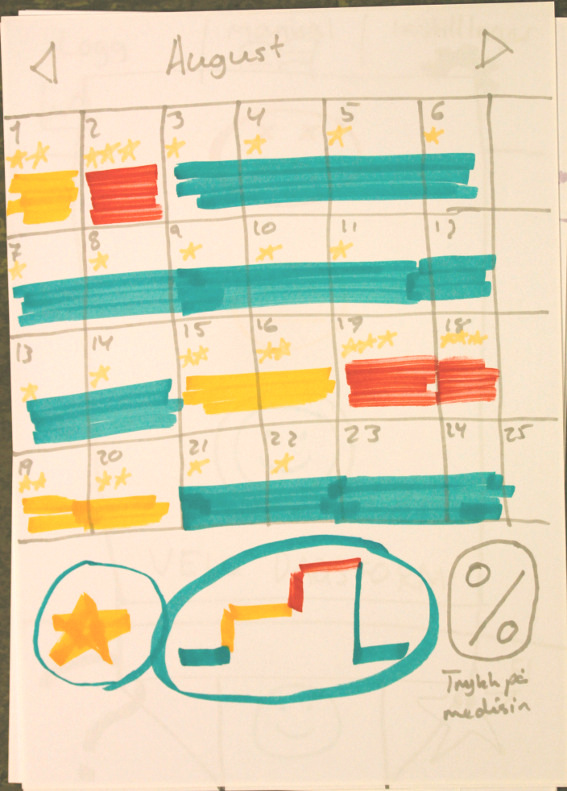
\includegraphics[width=7cm]{Pictures/DesignWorkshop/AdultLogView}
		\caption[Log view from design workshop]{View where adults can view the medication and health state history for a child.}
		\label{fig:dwAdultLogView}
	\end{center}
\end{figure}
\clearpage{}
\subsection{What was used in the further development}
Several ideas from the design workshop was used later in the development. We realized that we did not have sufficient time to make a very complicated distraction and
reward system for CAPP, so we decided to keep the ideas from the workshop about rewarding the child with stars whenever he or she completed a treatment.
This is easily implementable, and we believed it would be easy for parents to build on it with physical rewards when the child had accumulated enough stars.
For the same reasons we chose to keep and build on the idea of having an animation sequence where a Karotz avatar mirrored what the child had to do, it would
equip the inhalation mask when the child had to, making it more exciting for the child to do this as well. This approach have been seen to work with other applications,
like for helping children brush their teeth, and we wanted to use this as our base point.

We did the workshop based on the idea of having
one application, but later decided on having two. This meant that most of the basic GUI elements we came up with here, had
to be redone. For GAPP we implemented a log which kept its general layout, with the coloring showing which plan had been followed the relevant day. We later switched around on the additional information
that would be shown on each date and how, but the concept stayed the same.
\section{Frameworks used in the Project}
\label{sec:frameworks}
In this section the different frameworks that have been in use in the project is presented.
The frameworks consists mainly of the development model, the different programming languages, the 
database and server tools, the Karotz API, the Android SDK and the IDE used for development.


\subsection{Programming Languages, Message Formats and File Formats}
The following section will comment on different programming languages, communication protocols and 
file formats used in the project.

\subsubsection{Eclipse IDE}
\label{sec:Eclipse}
Eclipse \cite{Eclipse} is a multi-language software development environment comprising an integrated development environment (IDE) and an extensible plug-in system. The source code is mostly written in Java. Eclipse may be used to develop applications in Java and, by means of various plug-ins, other programming languages including Ada, C, C++, Ruby, Python, and many others. Eclipse is owned by the Eclipse Foundation, a non-profit organization focusing on creating and maintaining a community for individuals and organizations who wish to collaborate on commercially-friendly open source software. 

\subsubsection{Java}

Java is a programming language developed by Sun Microsystems in 1995, and is licensed under the GNU General Public License. 
Java can be run on any Java Virtual Machine (JVM), which means that it can run on any platform. It is an object oriented language and is based upon classes.
According to TIOBE Software (2012)\cite{TIOBE}, it was ranked as the 2nd most popular programming language in the world.


\subsubsection{Android SDK}
The Android software development kit (SDK) \cite{AndroidSDK} includes a comprehensive set of development tools used when developing Android software. The kit includes an Emulator, documentation of the source code, sample code, tutorials and a debugger. Enhancements to Android's SDK go hand in hand with the overall Android platform development. The SDK will also support older versions of the Android platform, through downloading extra packages of source code, in case developers wish to target their application towards older devices. By building the project through the IDE the Android application is packaged in a format which may be distributed (.apk). 

\subsubsection{Android Developer Tools}
The Android Developer Tools (ADT) \cite{AndroidADT} is a plug in for Eclipse that provides a professional-grade development environment for building Android applications. The ADT makes it easier to use the functions and tools that the Android SDK provides, by giving access through the user interface of Eclipse.


\subsubsection{Javadoc}
Javadoc is a tool for documenting code. It is integrated in Eclipse IDE, and we will use it document our code. When we use code-completion in Eclipse, the Javadoc of the function selected is shown as it's description.  

\subsubsection{JavaScript}
Two parts of the project will make use of JavaScript. The settings page for doctors is web based and 
will use JavaScript for interactivity. The Karotz can be programmed in two ways; either through a web 
API on the server side or through stored JavaScript code. In order to maximize stability and power, 
the client hosted JavaScript technique will be used.

JavaScript is a multi-paradigm, weakly typed and dynamic language that is extensively used on the web 
today. The main application of JavaScript is to enhance interactivity on a web page through client-side 
interpretation of the code in a browser. It can be used for a number of purposes such as making something 
happen when a button is pressed, loading new data without refreshing the page and much more. Even 
though JavaScript is by far most commonly used on the web there are also applications of it in other 
areas. Examples of these kinds of implementations are Node.js\cite{nodejs}, a network application creation
platform for writing JavaScript code as a regular server-side program, and the Karotz API which we will be 
using.

\subsubsection{Karotz API}
The Karotz API is based on a Javascript engine. The API is downloadable from the 
Karotz's homepage and gives access to the Karotz's different functions such as changing the color 
of the LED light, playing prerecorded sounds, waving it's ears and registering contact with an RFID-chip. 

A full documentation of the API is given, however most of the example code is commented in French.

\subsection{Database}
Since the project team has decided to use a database to store information relevant to the systems, there
is a requirement to use a programming language for creating and maintaining, as well as accessing, the
database. Because of technical limitations in the Karotz explained further in Section \ref{sec:databaseAccessLayer}
we chose to split the database into to parts: the database itself, written and maintained in MySQL, and
a set of access modules written in PHP (PHP: Hypertext Preprocessor) and MySQL.

\subsubsection{MySQL and phpMyAdmin}
MySQL\cite{mysql} is the world's leading open source database. It offers all the tools necessary to implement
and maintain data records for a project such as ours. The advantage of being the biggest contender is that there
is a myriad of resources easily and freely available to MySQL developers on the Internet. MySQL is suitable
for our project because it is reliable, free and open source, and all the group members have previous experience
working with it.

PhpMyAdmin is a graphical MySQL manager that is installed on NTNU's MySQL server\cite{ntnuphpmyadmin}. It provides
an easy way to manipulate a MySQL database without having to write any SQL code. Figure \ref{fig:phpmyadmin} shows
a typical screen from phpMyAdmin, where one can edit, add rows, add information etc. directly within a GUI. Since
NTNU's servers are already integrated with the program, and we use NTNU's MySQL server for development,
phpMyAdmin will be used to administer the database efficiently.

\begin{figure}
	\begin{center}
		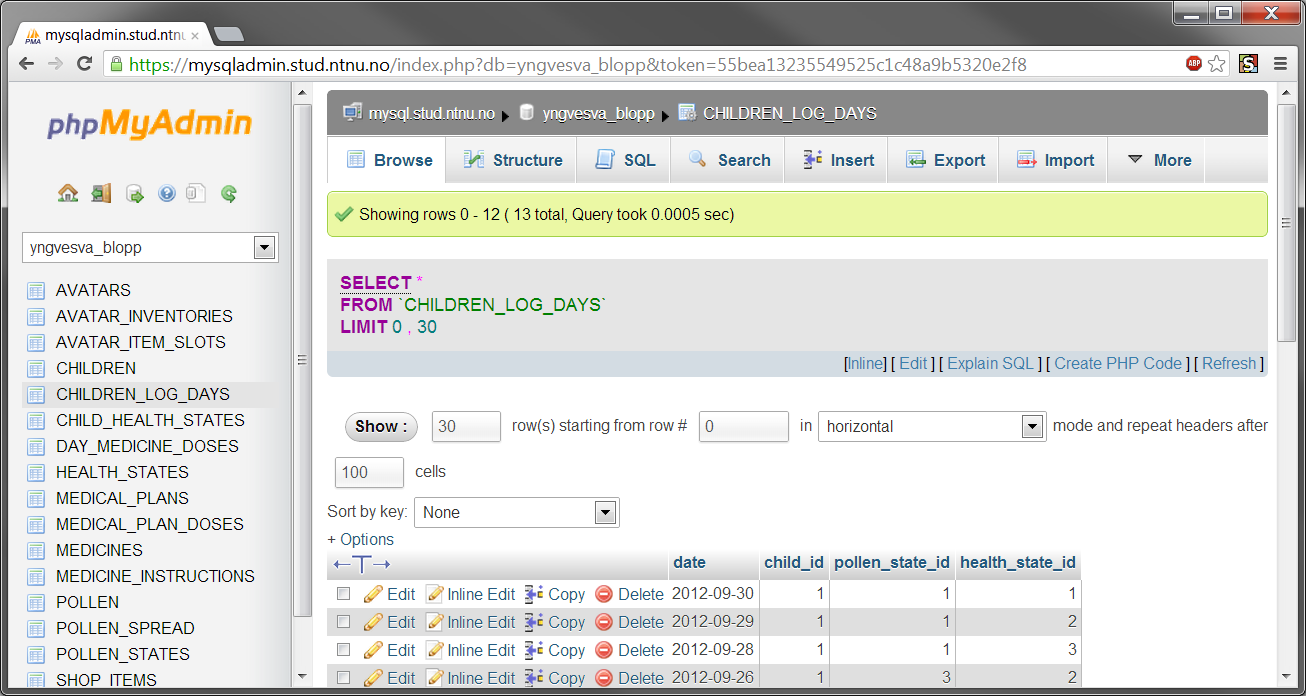
\includegraphics[width=17.5cm]{Pictures/Tools/PhpMyAdmin}
	\end{center}
	\caption{phpMyAdmin screenshot}
	\label{fig:phpmyadmin}
\end{figure}

\subsubsection{PHP}
PHP\cite{php} is a scripting language that is extensively used on the web because of its flexibility, ease of use
and popularity. It is mainly used for creating and editing HTML (HyperText Markup Language) pages server-side before sending to the client. In
our project, we used PHP to access the NTNU MySQL database from a web server located on a NTNU sub network(\url{http://folk.ntnu.no/}), 
and return a JSON file.

\subsubsection{JSON}
JSON\cite{json} is a format used for storing and sending data in a light, human-readable and easily parsable format.
It's based on JavaScript notation, but uses only a small subset of the JavaScript syntax; only strings, numbers, lists,
objects, booleans and the null value are included. We have used JSON for storing configuration data in the Karotz application, 
and for sending data between the PHP web access modules and the client applications.

\subsection{Extra Tools used in the Project}

The following section contains a description of the tools used for testing of the system, project and task 
management, team and customer collaboration, communication between participants. 
The tools chosen were chosen due to familiarity, making the learning curve as flat 
as possible. 

\subsubsection{Testing Tools}
This section describes tools used for performing unit tests, usability tests, and 
end-to-end tests.

\paragraph{HTTP Requests}
Postman\cite{postman} is a REST client for performing both basic and advanced HTTP requests to a
given URL. It is distributed as an extension for the \emph{Google Chrome} web browser. Postman keeps
a history of all sent requests, as well as an easy-to-understand interface for performing GET and
POST operations. Since the database was accessed through a web interface that used GET and POST methods,
it was natural to choose a REST client for the development process. Postman is also able to format
returned JSON, which was useful because the web access modules return JSON formatted data.
Figure \ref{fig:postman} shows a typical screen in Postman when performing a POST operation.

\subsubsection{Dropbox}
For file sharing between customer and the developer team, and the developer team 
between each other, we used Dropbox. Dropbox\cite{dropbox} is an online storage which 
allows sharing of folders and documents between invited partners. Dropbox is 
asynchronous, meaning only one person may edit a document at a time.

\subsubsection{Git}
To ensure that every team member was always up to date and no documentation was lost, 
version control systems were enforced. Git\cite{git} was used as a tool for version 
control. Git is a distributed source code management system, and was developed by Linus Torvalds in 2005. 
It comes with a lot of useful features like rollbacking to previous versions, file history and possibility to work on several branches, among others. 
The repository was hosted at Github (\url{http://github.com}). 

\subsubsection{Google Drive}
Google Drive (earlier Google Docs), is a file storage and synchronization service made by Google. Google Docs is now housed at Google Drive, and is 
a free web-based office suite. Google Docs allows several individuals to share and write the same document at the same time, and is ideal to write
simple documents concurrently.
Google Drive was used for writing agendas and status reports.


\begin{figure}
	\begin{center}
		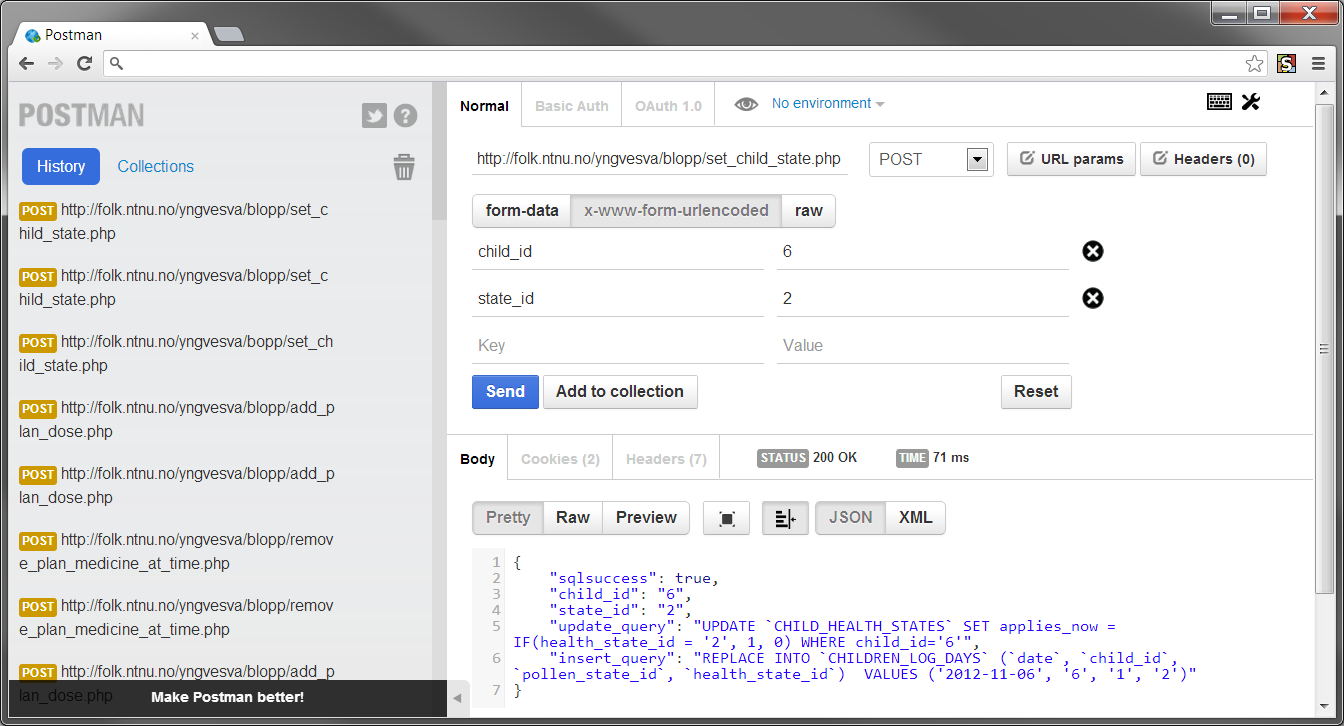
\includegraphics[width=17.5cm]{Pictures/Tools/Postman}
	\end{center}
	\caption{Postman screenshot}
	\label{fig:postman}
\end{figure}

% \subsection{Task Management, Collaboration and Communication Tools}
% The following section contains a description of the tools used for project and task 
% management, team and customer collaboration and communication between participants. 
% The tools chosen were chosen due to familiarity, making the learning curve as flat 
% as possible. 
% 
% For file sharing between customer and the developer team, and the developer team 
% between each other, we used Dropbox. Dropbox\cite{dropbox} is an only storage which 
% allows sharing of folders and documents between invited partners. Dropbox is 
% asynchronous, meaning only one person may edit a document at a time.
% 
% To ensure that every team member was always up to date and no documentation was lost, 
% version control systems were enforced. This way the information we made sure that an 
% online backup existed, in case of errors occuring. Git was used as a tool for version 
% control. 

\subsubsection{Task Management}
To ensure task management the team used AgileZen. AgileZen\cite{agilezen} is an online 
project management tool. You can add user stories, build a backlog and easily add 
tasks to each story. Unfortunately it is not perfect for projects using 
Scrum. AgileZen gives no simple way of keeping order of which task is to be done within a certain sprint. 
Their suggestion is using color coding of tasks, but this was not preferable.
There is also no way to assign a single task to a person, you may only sign epics/user stories to a user. Leaving no opportunity for showing that two people may work at the same use story at the same time. At a small project, such as ours this was at times a necessity, which AgileZen did not fulfill.
The team used AgileZen in order to keep the customer updated, while the team 
used Google Docs internally in order to keep track of tasks. 

\subsubsection{Mockup Tool}
For mockups the team chose Balsamiq Mockups. Balsamiq Mockups\cite{balsamiqmockups} is 
a tool designed for easing the collaboration between the GUI developers and the customer. 
The main advantage to Balsamiq Mockups is the way it ensures no one is too attached to the 
design. By making sketchy, low-fidelity frames it moves the focus of design conversations 
towards functionality. Balsamiq also has functionality for making click-through prototypes, 
which are very nice for demonstration purposes and usability testing. The team was also 
advised by the customer and the advisor to use Balsamiq Mockups.

\subsection{Design Principles}
Google\cite{androidguidelines}, who is developing the Android operating system has some design 
principles in order to help programmers make better applications. As Google 
states, quotation: "These design principles were developed by and for the Android User 
Experience Team to keep users' best interests in mind. Consider them as you apply your 
own creativity and design thinking. Deviate with purpose."

Many of these principles are guidelines to help the developers make more attractive 
and better applications, and some of them are rules, meant to follow without deviation. 
Google does not always state which is which, but refers to their slogan ``Don't be evil'', 
meaning developers should not try to scam, trick or hurt users through their applications.

The team as a group has read the design principles and would like to mention the ones that 
are most central for the applications we are making: 
\begin{description}
	\item[Real objects are more fun than buttons and menus.] The principles states that users should directly touch and manipulate objects, rather than 
	buttons and menus. This reduces the cognitive effort needed to perform a task while making 
	it more emotionally satisfying.
	\item[Let me make it mine.] People love to add personal touches because it helps them feel at home and in control. 
	Provide sensible, beautiful defaults, but also consider fun, optional customizations 
	that don't hinder primary tasks.
	\item[Keep it brief.] Use short phrases with simple words. People are likely to skip sentences if they're long.
	\item[Only show what I need when I need it.] People get overwhelmed when they see too much at once. Break tasks and information into 
	small, digestible chunks. Hide options that are not essential at the moment, and teach 
	people as they go.
\end{description}



\section{Software Architecture}
In this section, we'll describe some of the software architecture concepts that is applied in the development of the project.
``The software architecture of a system is the set of visible structures needed to reason about the system, which comprise software elements, relations among them, and properties of both." \cite{bassclemetskazman}
 
 
\subsection{MVC - Model View Controller}
\label{sec:mvcintro}
MVC is an architectural pattern used frequently in small software systems and applications similar to CAPP and GAPP.
The pattern consists of three components, Model, View, and Controller respectively.

A model consists mainly of ``raw'' data. A view is responsible to display the data to a user in an appropriate manner, while the controller receives input and manipulates the data models 
given the input. 

We will use MVC as our main architectural pattern to develop CAPP and GAPP. 
  
The advantage of using MVC in applications is that it separates functionality, and it becomes easier to modify the functionality of for instance a single underlying models. 


Figure \ref{fig:diagram-mvc} shows an textual image of MVC. An arrow from A to B indicates an association from A to B.
\begin{figure}
	\centering
		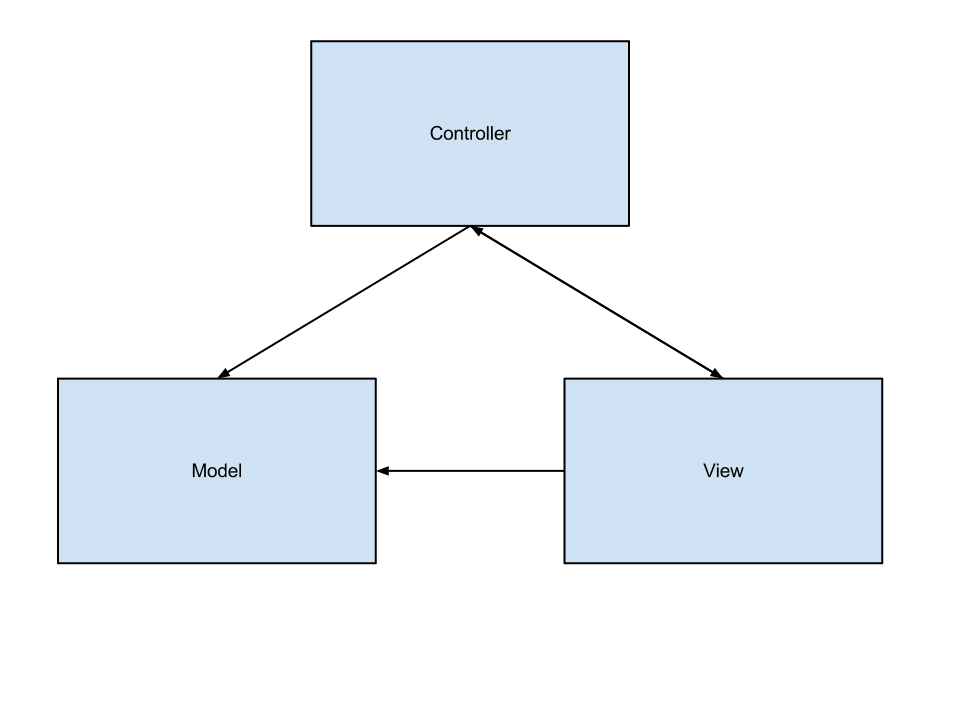
\includegraphics[width = 17.5 cm]{Pictures/ArchPictures/MVC.png}
	\caption{Graphical view of MVC}
	\label{fig:diagram-mvc}
\end{figure}

\subsection{4+1 View Model}
\label{sec:viewmodel}
Kruchten (1995)\cite{4+1viewmodel} defines the 4+1 View Model as a model for describing the software architecture for
several stakeholders through different views (Please note that ``View Model'' in this context is something completely different than the views and models described in Section 
\ref{sec:mvcintro}). These views are called Physical
View, Process View, Development View and Logical View, respectively, and are built around a series of scenarios, or use cases. 
We will use this model to describe the architecture in Chapter \ref{chap:systemDesign}

Table \ref{tab:4plus1ViewModel} shows the purpose of the different views.

\begin{table}
	\centering
	\begin{tabular}{|p{0.3\linewidth} |p{0.6\linewidth}|}
		\hline View & Purpose \\
		\hline Logical & The logical view is an object model of the design, and is concerned with end user functionality. 
		Addresses end users, customer and development team to give a brief introduction to how the system is implemented.\\
		\hline Process & The process view gives a description of concurrency and synchronization aspects of the design. Reflects upon properties like scalability, performance, and internal processes. \\ 
		\hline Physical & Describes how the system interacts with different types of hardware. Addresses system engineers, and describes communication protocols and topology. \\
		\hline Development & Describes how the software is organized in a development environment. Addresses programmers and software management. \\
		\hline 
	\end{tabular}
	\label{tab:4plus1ViewModel}
	\caption{Purpose of the 4+1 View Model}
\end{table}


  


\section{Privacy and security}
Early in the project we did some research into what information we could be legally allowed to keep track off, and 
more importantly, what was recommended to avoid doing, to be able to avoid issues later. Specifically we looked into
what information we could save regarding how well the medicationplans were followed, and in if this information could
be sent to medical staff, with information about who followed the plans well and who did not. We discovered it was not
necessarily legal to send this information without consent from the person the data was collected from, or in our case, 
the guardian of that person. We thought about making this information 
available to medical staff, but dropped it since it is illegal to send
this type of information without consent.

In terms of whether or not we could use the child's personal number as an identifier, we discovered that this was legal, but only 
if we had an actual need to save it, that we had pursuant in the law to save it, and finally, that satisfactory identification 
of the relevant person could not be achieved in any other way. For the system we were making we had none of these 
criteria in order, but for future expansions this might be information actually required. Hospitals have to be sure they 
give medicines to the correct people, so the personal number is already written on any prescription medicine used. If the 
system is expanded towards the hospital nebulization treatment it might be necessary or useful to store the personal number
in our database, to connect the user with the person receiving the treatment.

